\onecolumn
\section{Additional plots}
\label{sec:additional_plots}

\begin{figure}[H]
    \centering
    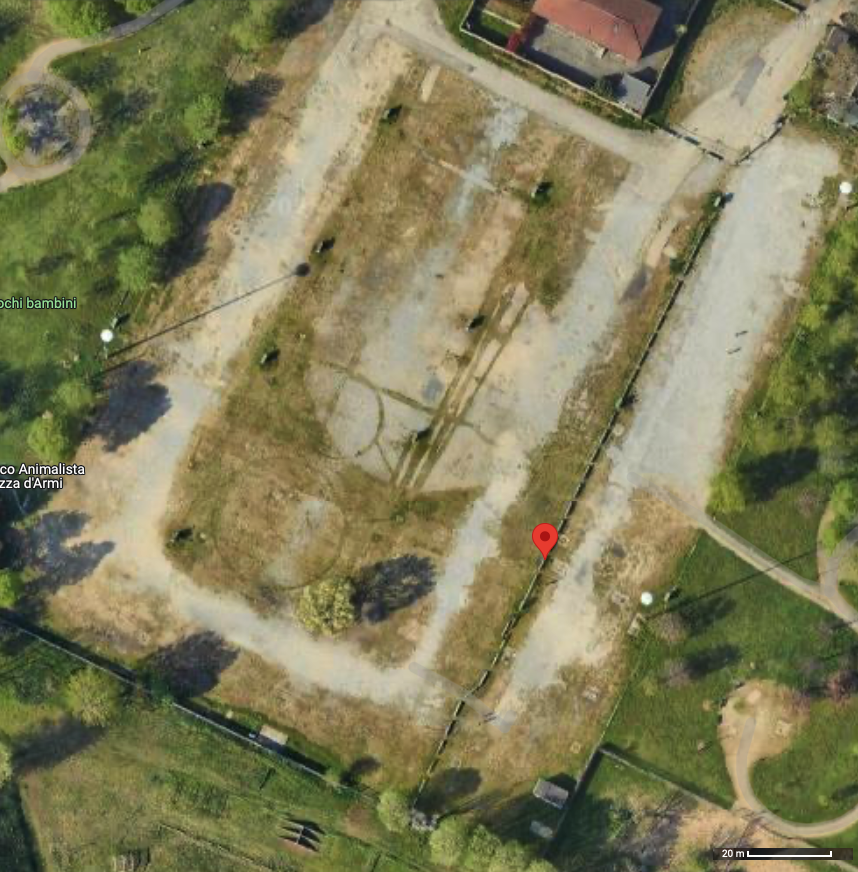
\includegraphics[width=0.5\linewidth]{images/map_place.png}
    \caption{Place where all surveys were carried out.}
    \label{fig:map}
\end{figure}

% \begin{figure}[H]
%     \centering
%     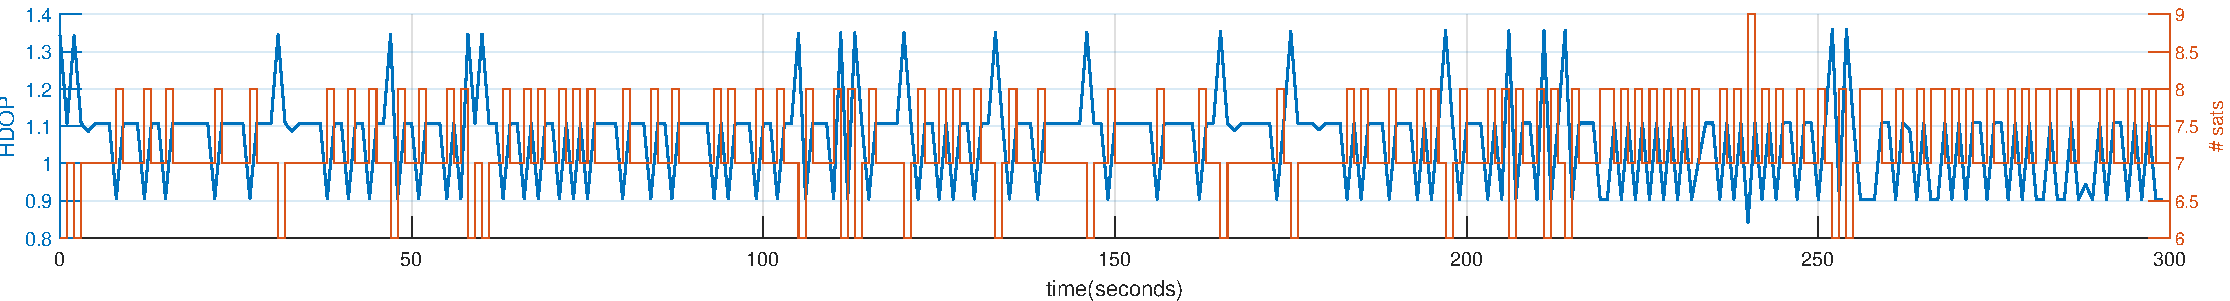
\includegraphics[width=1.00
%     \linewidth]{images/carne_hdop_carne.pdf}
%     \caption{HDOP and SATs number in the interference scenario}
%     \label{fig:carne_hdop}
% \end{figure}

\begin{figure}[H]
    \centering
    \begin{minipage}[b]{0.48\linewidth}
        \centering
        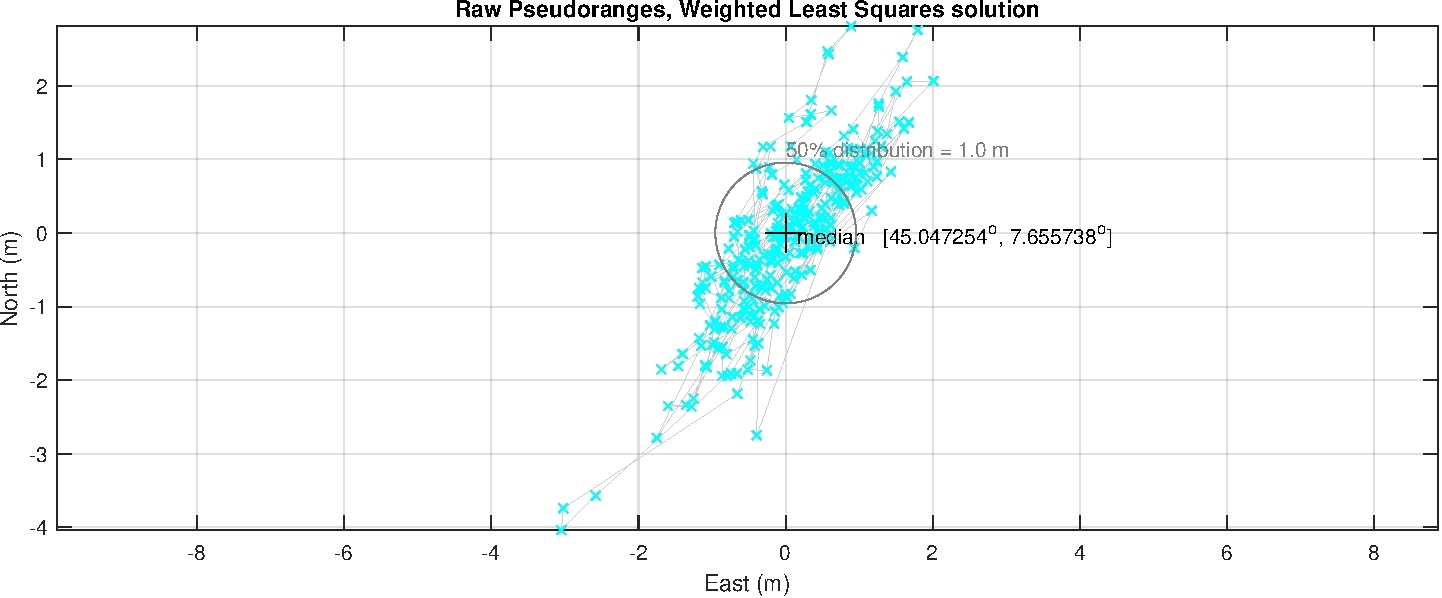
\includegraphics[width=1.00\linewidth]{images/pos_punto_3_precision.pdf}
        \caption{Positioning geoplot for logs collected in open-sky conditions (\ref{sec:opensky})}
        \label{fig:pos_punto_3_precision}
        \end{minipage}
    \hfill
    \begin{minipage}[b]{0.48\linewidth}
        \centering
        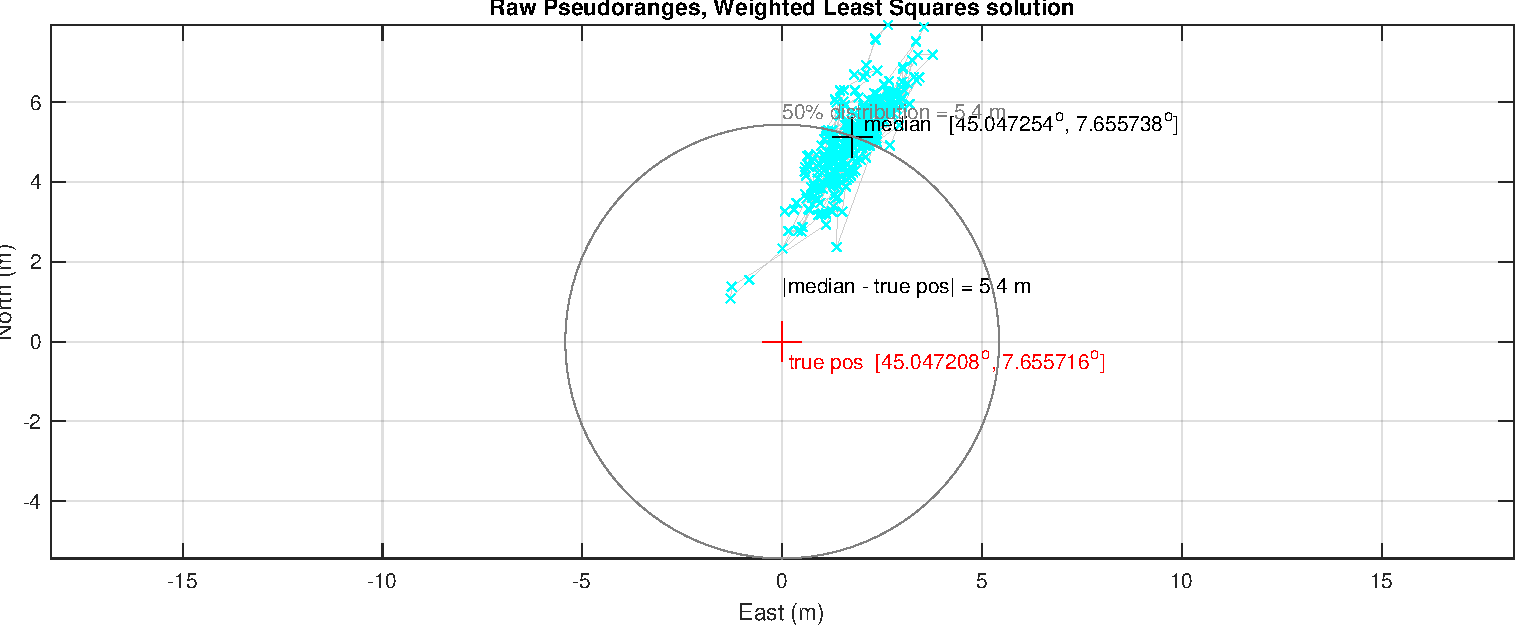
\includegraphics[width=1.00\linewidth]{images/pos_punto_3.pdf}
        \caption{Positioning geoplot for logs collected in open-sky conditions, correlated with true position (\ref{sec:opensky})}
        \label{fig:pos_punto_3}

    \end{minipage}
\end{figure}

\begin{figure}[H]
    \centering
    \begin{minipage}[b]{0.48\linewidth}
        \centering
        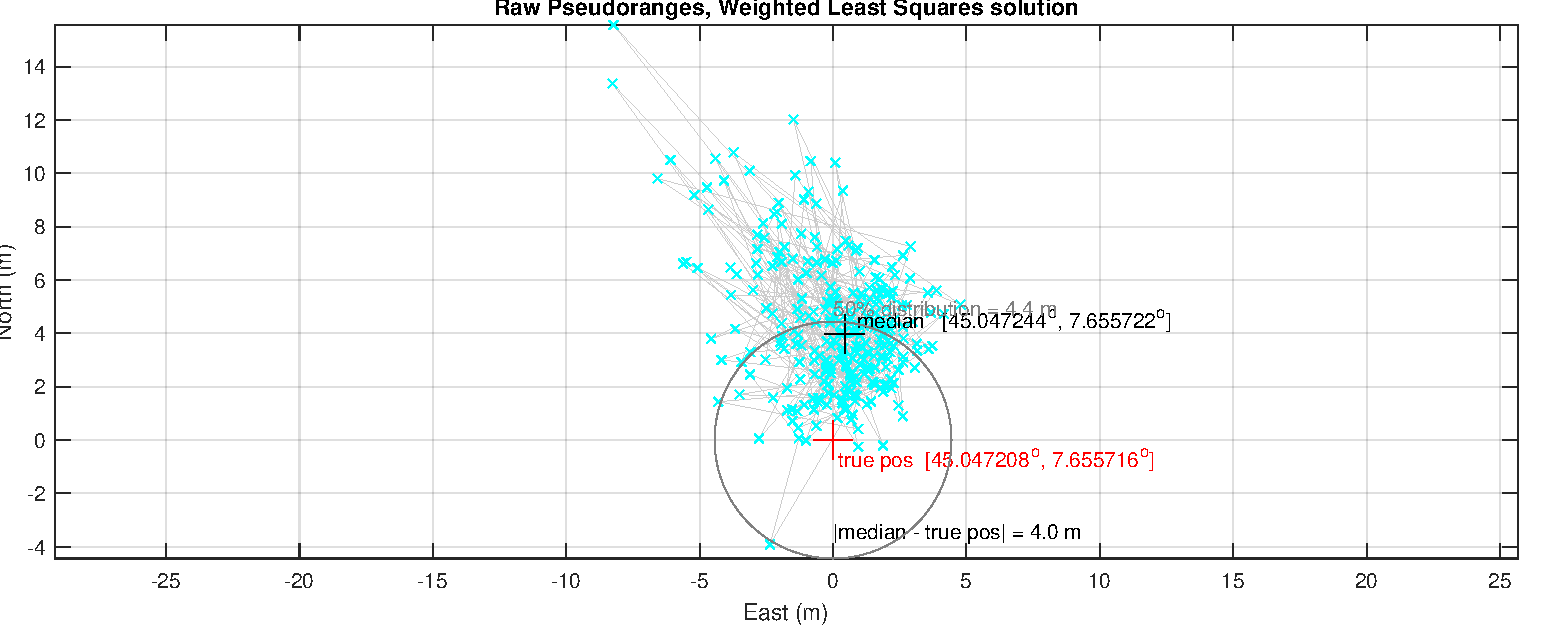
\includegraphics[width=1.00\linewidth]{images/carne_pos.pdf}
        \captionsetup{labelformat=empty}
        \caption{\textbf{Figure \ref{fig:carne_pos}:} Positioning geoplot for logs collected in the interference scenario (\ref{sec:opensky})}
        \end{minipage}
    \hfill
    \begin{minipage}[b]{0.48\linewidth}
        \centering
        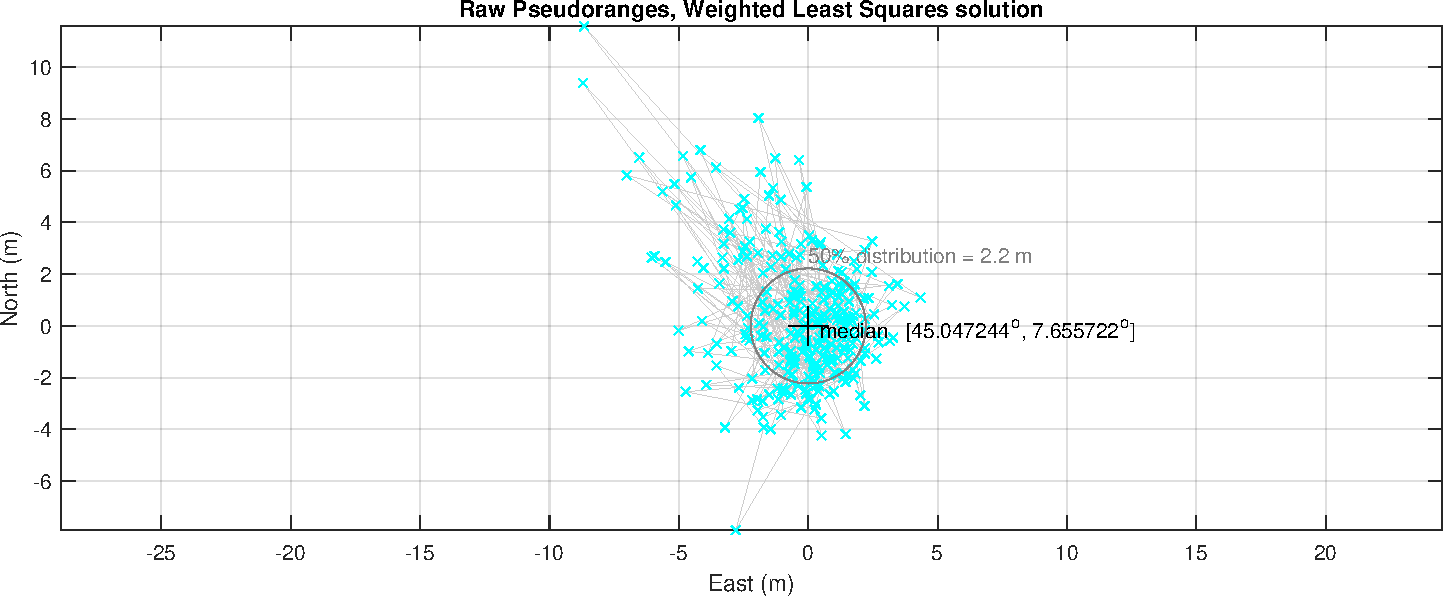
\includegraphics[width=1.00\linewidth]{images/carne_pos_precision.pdf}
        \caption{Positioning geoplot for logs collected in the interference scenario, correlated with true position (\ref{sec:opensky})}
        \label{fig:carne_pos_precision}

    \end{minipage}
\end{figure}


\begin{figure}[H]
    \centering
    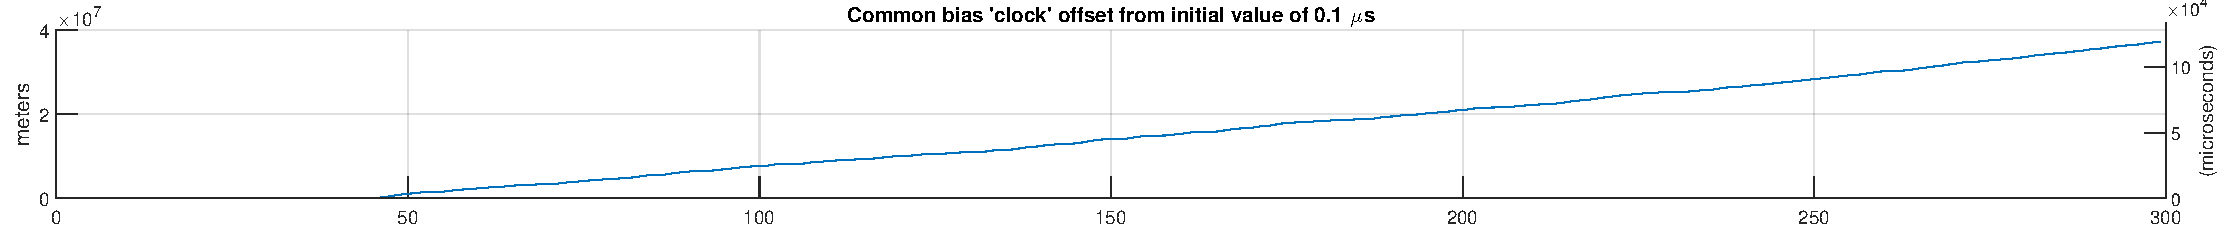
\includegraphics[width=0.95\linewidth]{images/discontinuity_bias_clock.pdf}
    \caption{Common bias clock offset in HW clock discontinuity} 
    \label{fig:discontinuity_bias_clock}
\end{figure}

\begin{figure}[H]
        \centering
        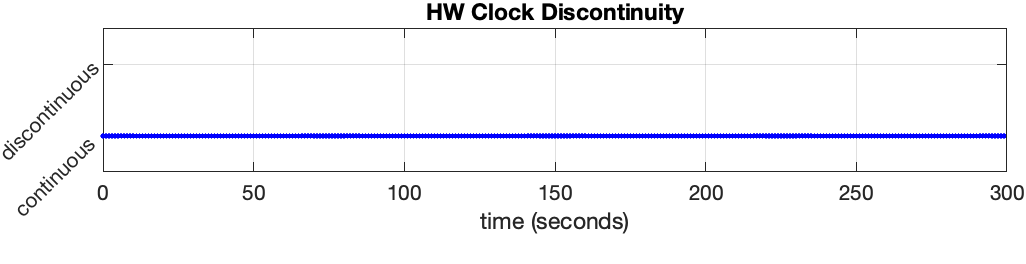
\includegraphics[width=0.85\linewidth]{images/continuity_gnss_log.png}
        \caption{Status of the GNSS hardware clock over time with GNSSLogger and GPSTest in parallel}
        \label{fig:GNSSLogger-continuity}
\end{figure}

\begin{figure}[H]
    \centering
    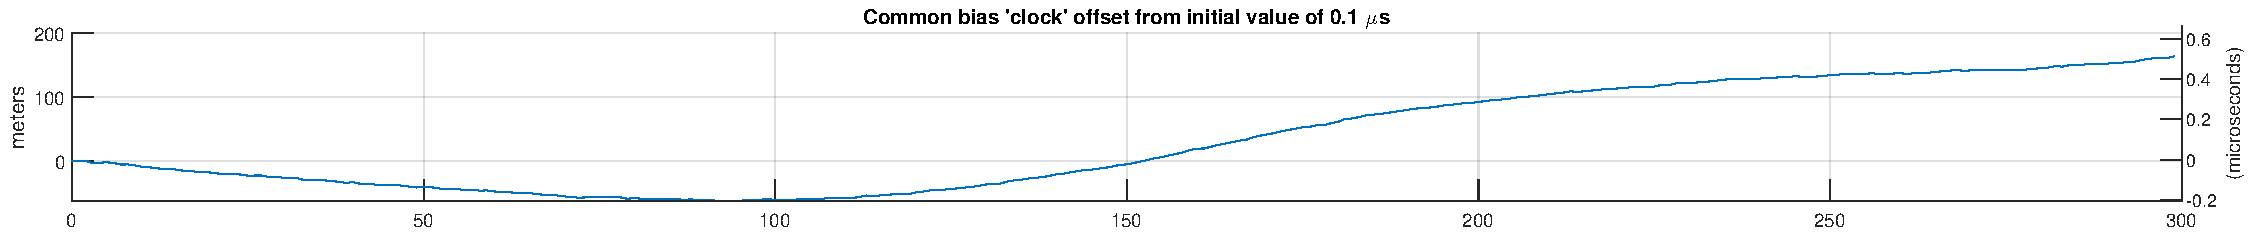
\includegraphics[width=0.95\linewidth]{images/continuity_bias_clock.pdf}
    \caption{Common bias clock offset in open-sky and HW clock continuity conditions (\ref{sec:opensky})} 
    \label{fig:continuity_bias_clock}
\end{figure}


\begin{figure}[H]
    \centering
    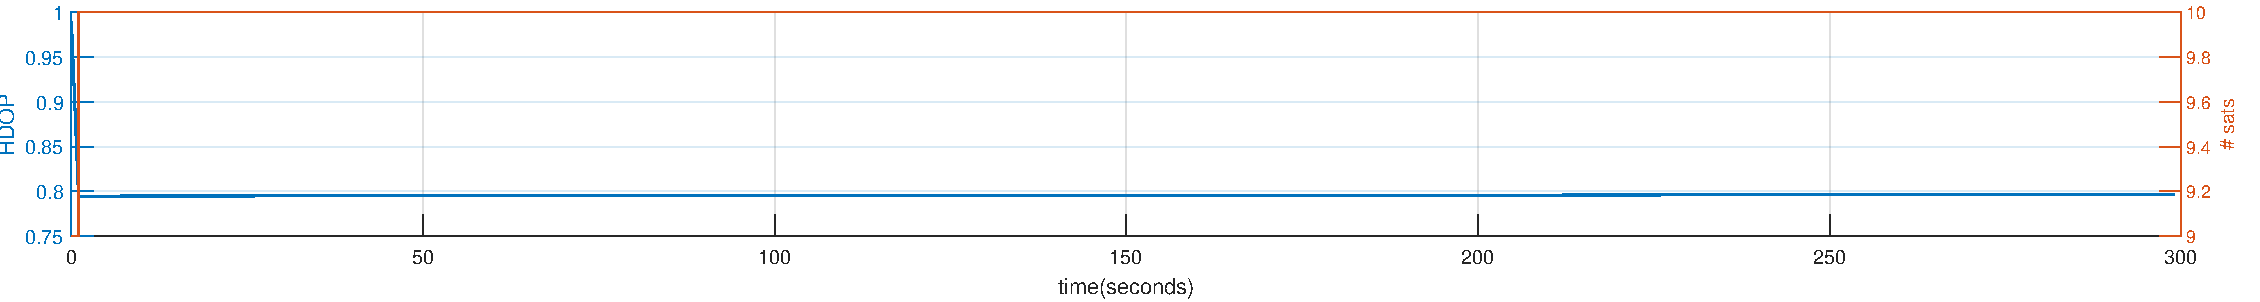
\includegraphics[width=1.00
    \linewidth]{images/hdop_punto_3.pdf}
    \caption{Horizontal diluition and number of satellites for logs collected in open-sky conditions (\ref{sec:opensky})}
    \label{fig:hdop_punto_3}
\end{figure}

\begin{figure}[H]
    \centering
    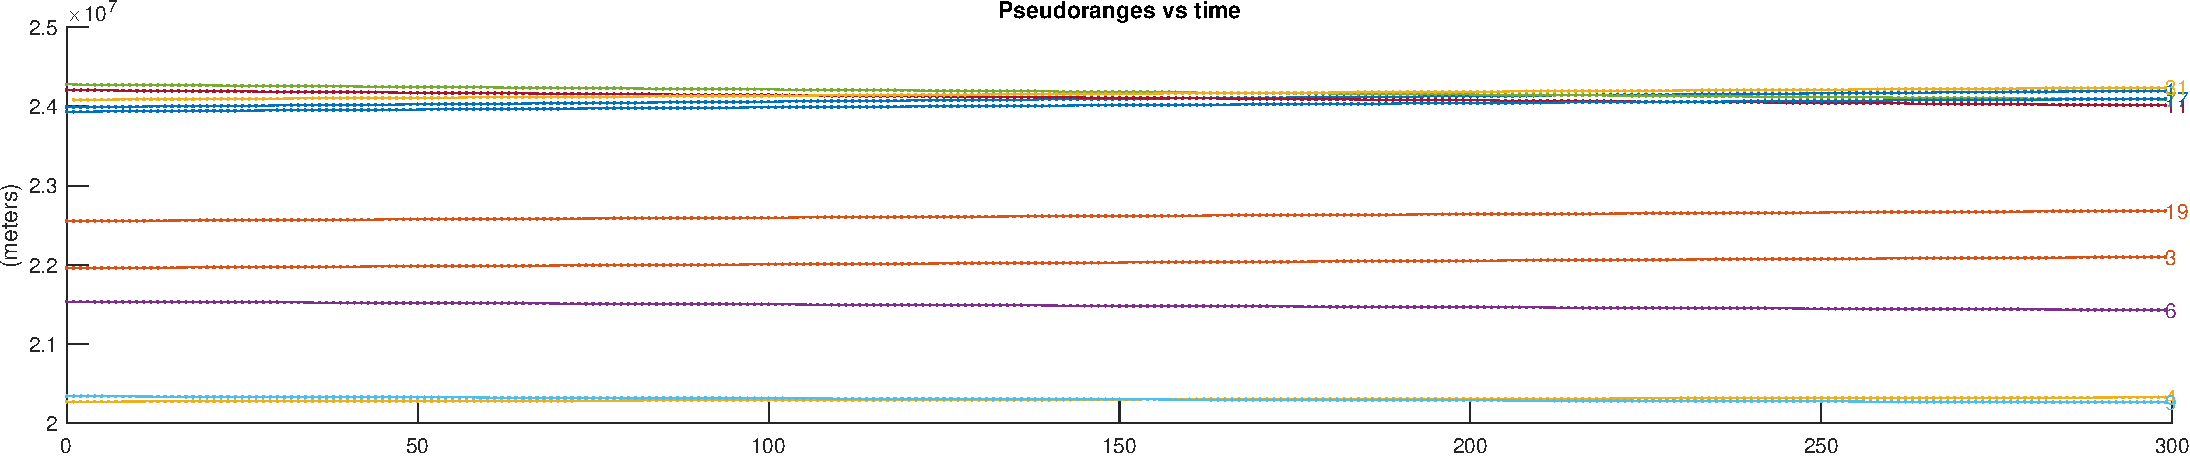
\includegraphics[width=1.00
    \linewidth]{images/punto3_pseudoranges.pdf}
    \caption{Pseudoranges vs. time for logs collected in open-sky conditions (\ref{sec:opensky})}
    \label{fig:pseudoranges_opensky}
\end{figure}

\begin{figure}[H]
    \centering
    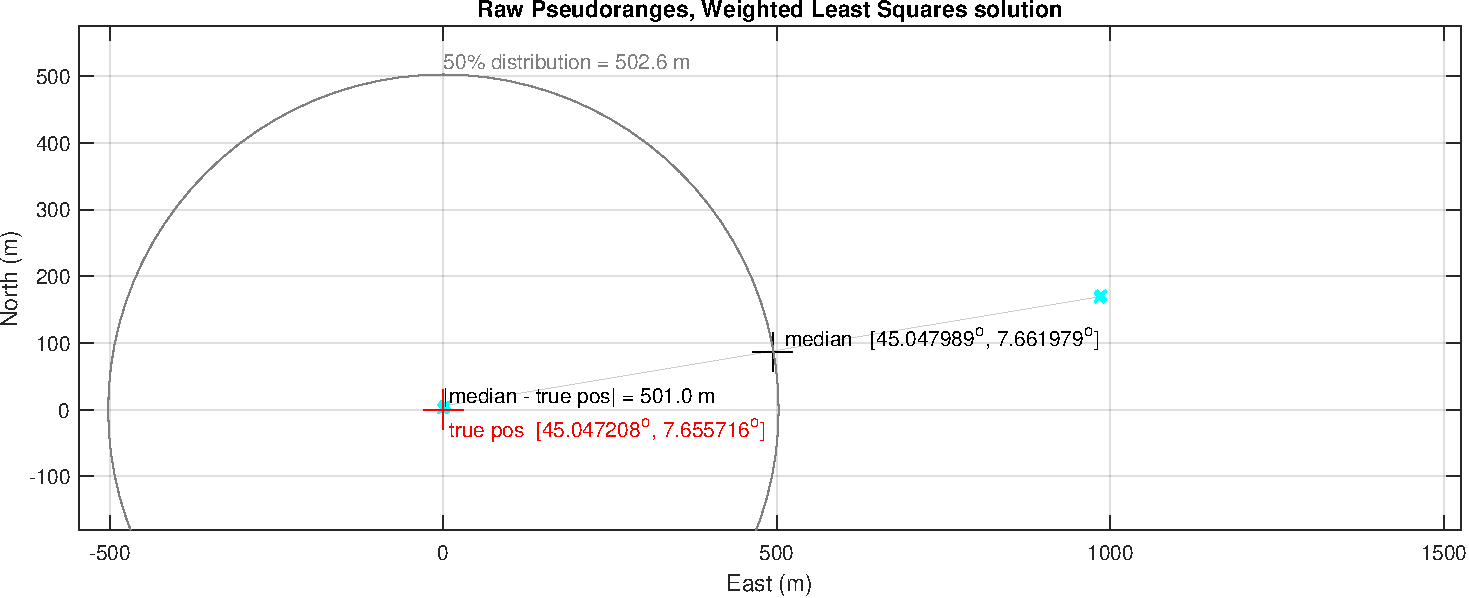
\includegraphics[width=1.00
    \linewidth]{images/pos_spoofed_no_delay.pdf}
    \caption{Positioning geoplot after applying spoofing to a location 1 Km from the real one, with no additional time delay used}
    \label{fig:pos_spoofed_no_delay}
\end{figure}

\begin{figure}[H]
    \centering
    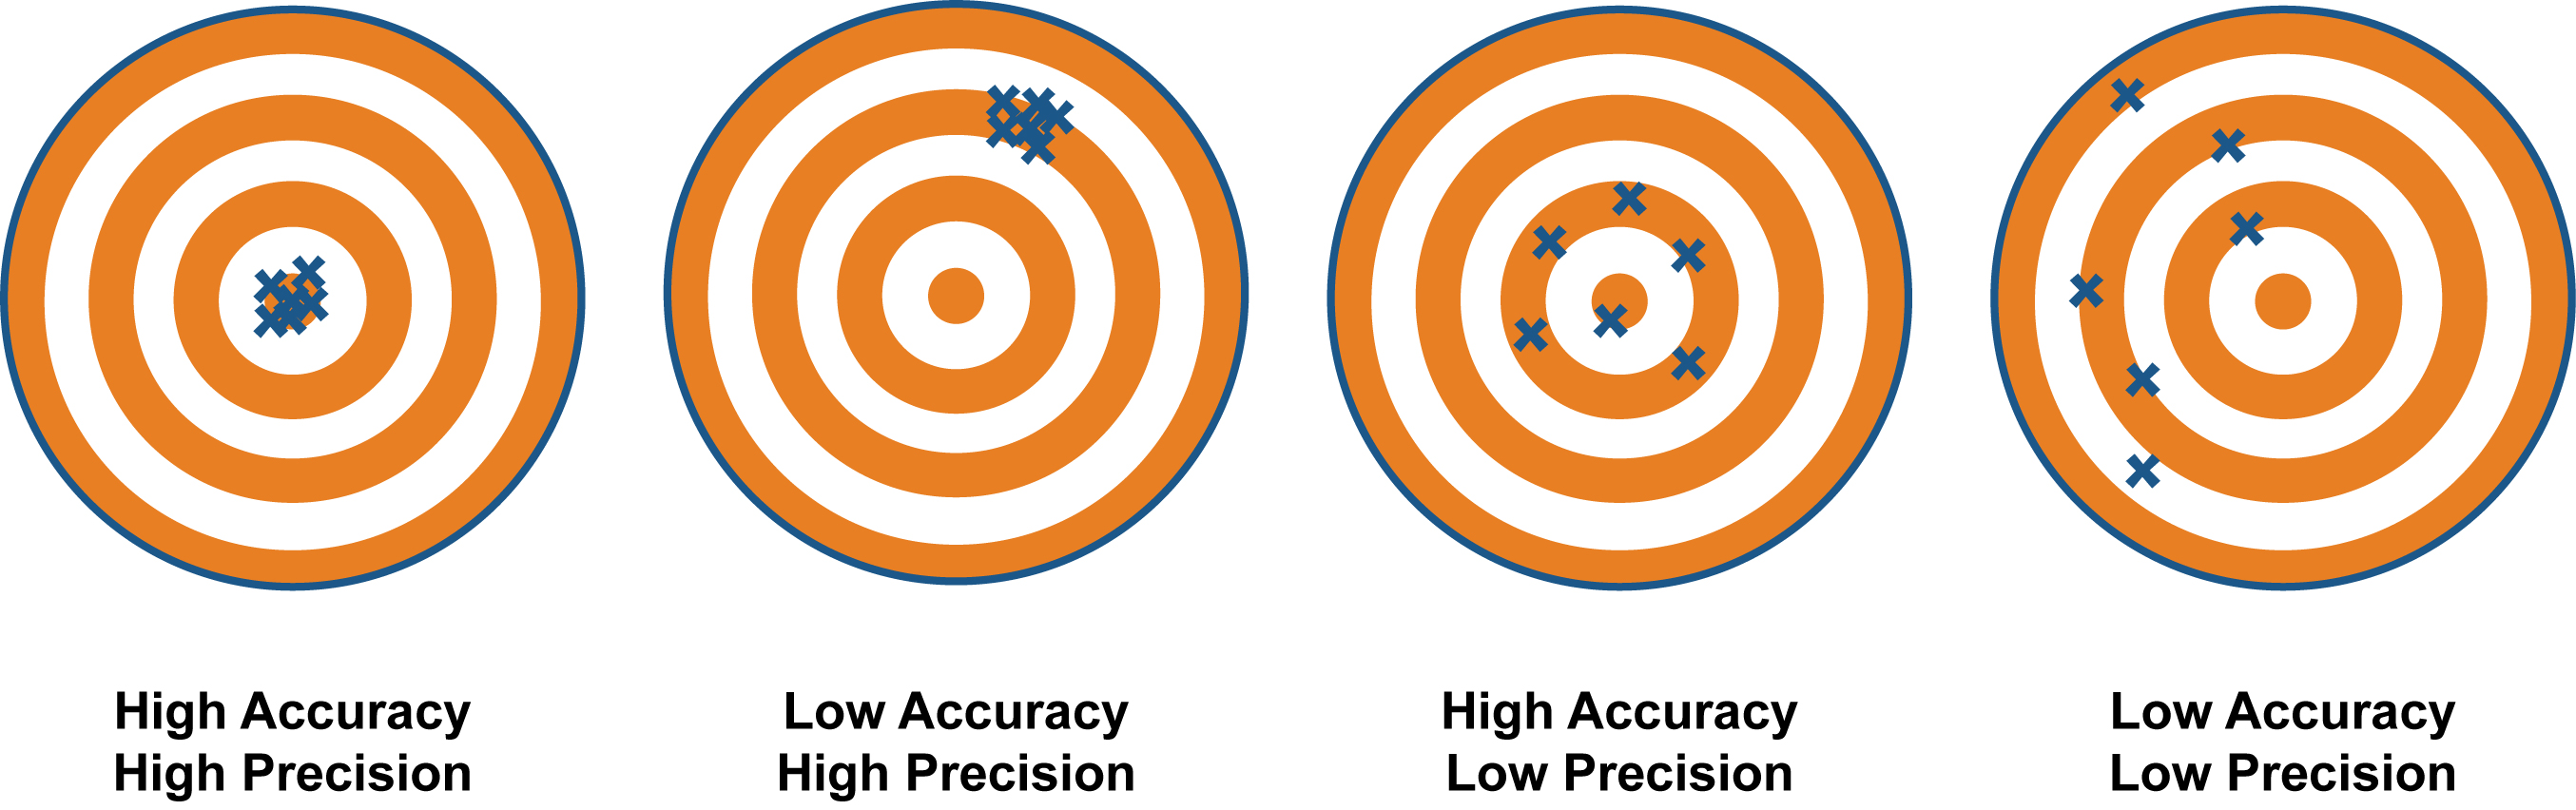
\includegraphics[width=0.50
    \linewidth]{images/Accuracy-vs-precision1.jpg}
    \caption{Accuracy vs. Precision}
    \label{fig:accPos}
\end{figure}

% \section{Appendix section title}
% \label{sec:underwater-comm}
% \colorbox{yellow}{Do we need this?}

% \begin{minted}[fontsize=\small, breaklines]{python}
% import subprocess
% import time
% import numpy as np
% import csv

% def run_iperf(name, server_ip, bind_ip, reverse, repetitions, pcap_fileNoExt, server_port, duration, udp, bitrate, app_buff_length):
% \end{minted}
